\documentclass[12pt]{article}
\usepackage{setspace}
\setlength{\parindent}{4em}
\usepackage{fancyvrb}
\usepackage{graphicx}
\usepackage{geometry}
\renewcommand\thesection{\arabic{section}}
\renewcommand\thesubsection{\thesection.\arabic{subsection}}
\geometry{letterpaper, portrait, margin=1in}

%%%Title Page%%%
\title{\vspace{3cm}Lab 05\bigbreak Assembling the Processor}
\author{
{\normalsize
\begin{tabular}{l r r}
 & \textbf{Ryan Cruz} & \textbf{Zachary Davis}\\
\textbf{Category} & ryan.cruz25@uga.edu & zachdav@uga.edu\\
\hline
Pre-lab 						  & 50 & 50\\
In-lab Module \& Testbench Design & 50 & 50\\
In-lab Testbench Sim. \& Analysis & 50 & 50\\
In-lab FPGA Synthesis \& Analysis & 50 & 50\\
Lab Report Writing 				  & 50 & 50\\
\end{tabular}
}}
%%%%%%%%%%%%%%%%%

\begin{document}
\maketitle
\newpage
\setstretch{2.5} % for custom spacing
\tableofcontents
\setstretch{1} % for custom spacing
\newpage

\section{Lab Purpose} \vspace{-.7cm} \line(1,0){470}
	\paragraph{}
		Entering this lab, we now have all of the components to complete the design of the Toy Processor. The two main modules that have resulted from our previous labs are the datapath and the controller. In this lab, we will connect those two components and then test its behavior with a simple program by encoding certain instructions and executing them in a test fixture to view data inputs and their respective outputs. 
		
\section{Implementation Details} \vspace{-.7cm} \line(1,0){470}
		\subsection{Prelab}
			\hfill

		\begin{figure}[h]
		\centering
			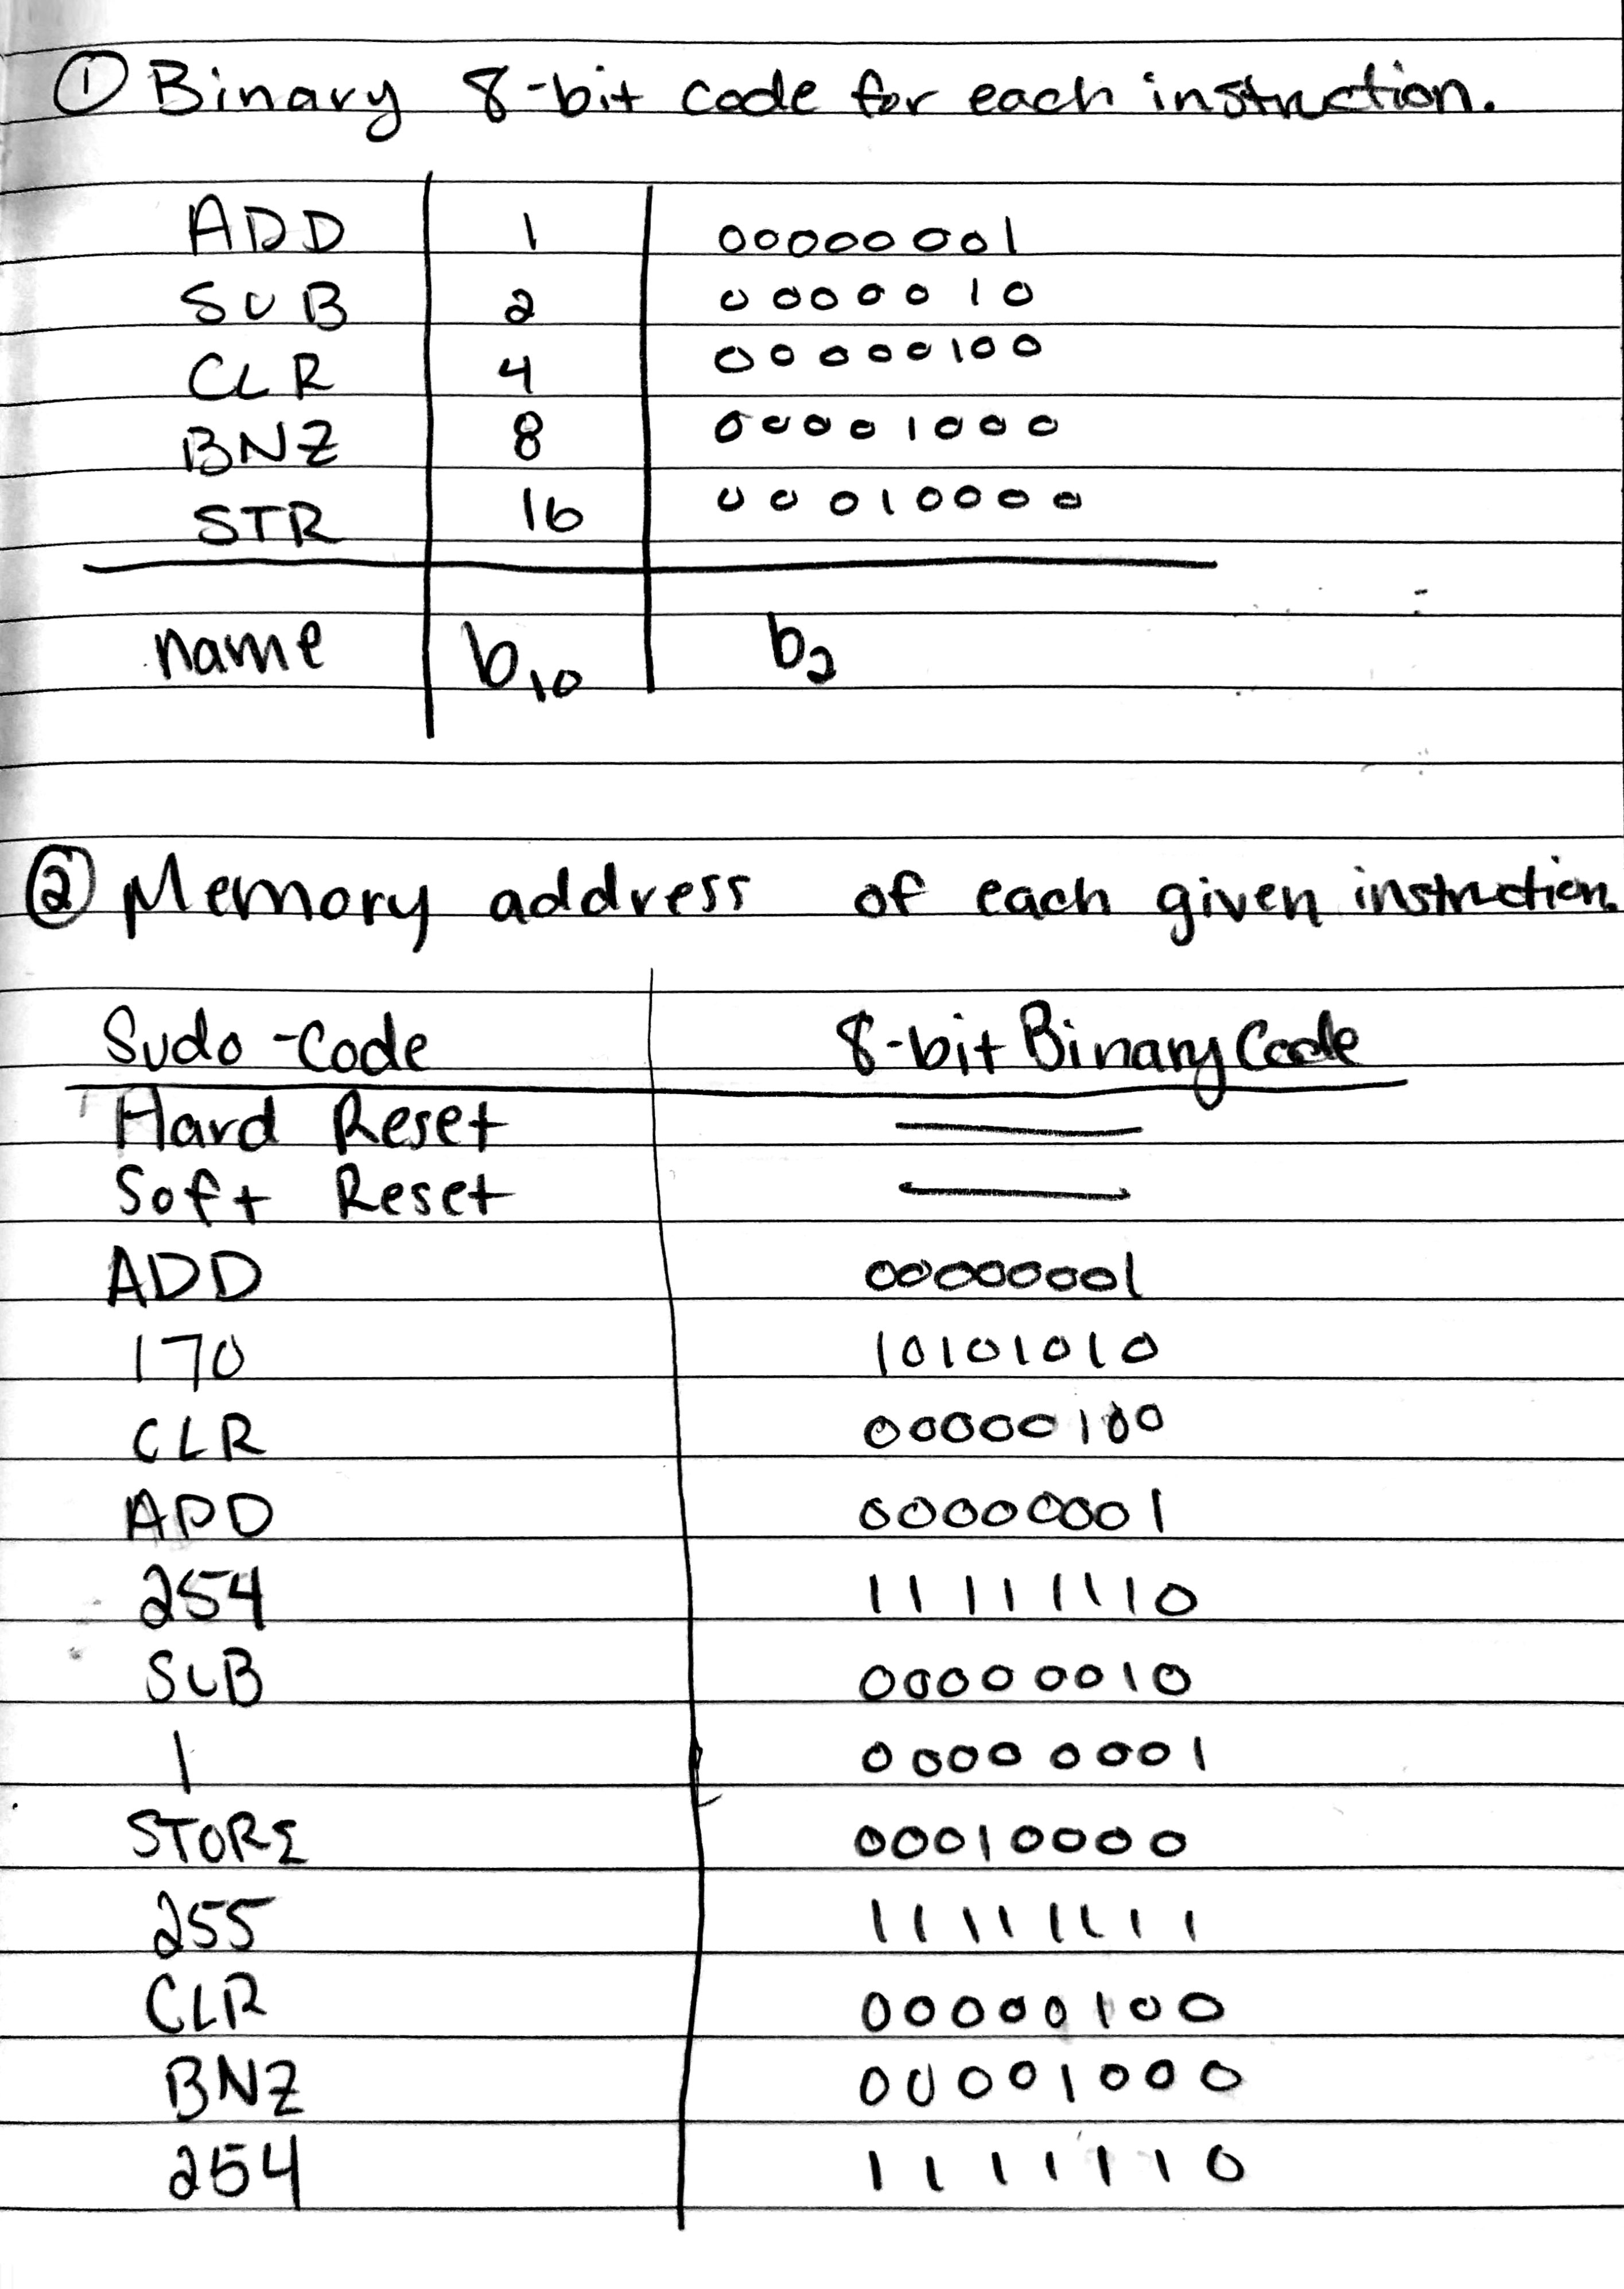
\includegraphics[scale=.09]{Prelab.jpg}
			\caption{The Binary 8-bit code for each instruction, as well as the memory addresses for each given instruction.}
		\end{figure}

		
\newpage
	\subsection{Circuit Implementation in Schematic Editor}
		\paragraph*{}
			
		\begin{figure}[h]
			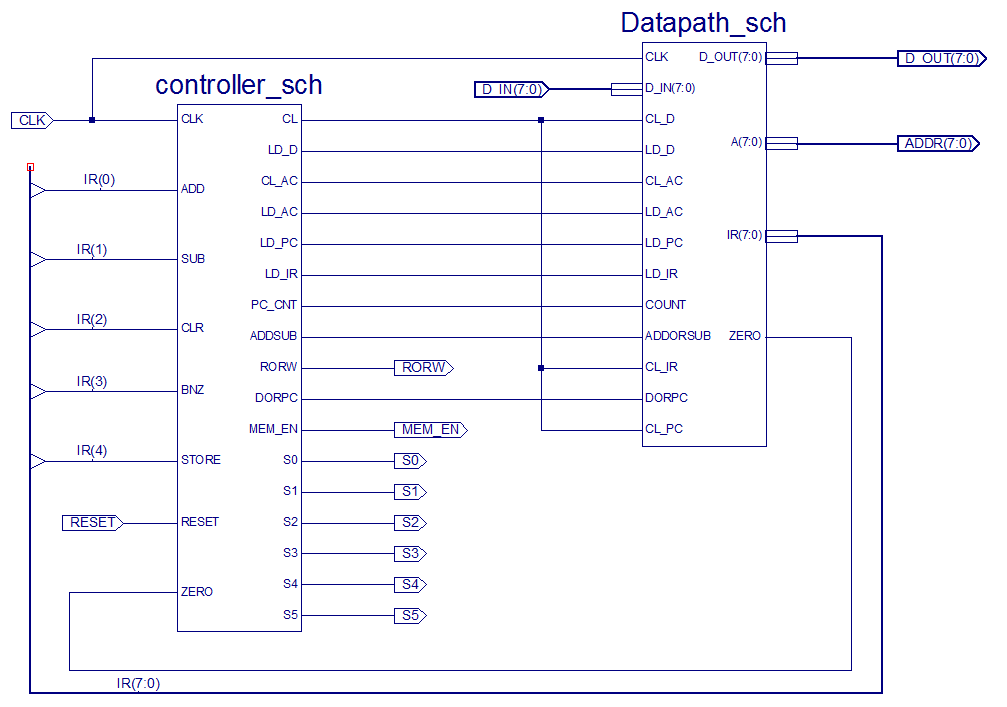
\includegraphics[scale=.6]{toy_sch.PNG}
			\caption{Controller and Datapath components from previous labs connected here in toy\_sch.}
		\end{figure}
		
		\newpage
	\subsection{Simulation}
		

		
		\begin{Verbatim}[frame=single, fontsize= \small]
//toy_tb.v
`timescale 1ns/1ps

module toy_tbw_tb_0;

	reg CLK = 1'b0;
	reg [7:0] D_IN = 8'b00000000;
	reg RESET = 1'b1; 

	wire [7:0] ADDR; 	
	wire [7:0] D_OUT; 
	wire MEM_EN;
	wire RORW; 
	wire S0;
	wire S1;
	wire S2;
	wire S3; 
	wire S4; 
	wire S5;

	initial // Clock process for CLK 
		begin 
			forever 
				begin
					CLK = 1'b0;
					#50; 
					CLK = 1'b1; 
					#50;
				end 
		end
		
	toy_sch UUT ( 
	.CLK(CLK), 
	.D_IN(D_IN),
	.RESET(RESET),
	.ADDR(ADDR), 
	.D_OUT(D_OUT), 
	.MEM_EN(MEM_EN), 
	.RORW(RORW), 
	.S0(S0),
	.S1(S1), 
	.S2(S2), 
	.S3(S3), 
	.S4(S4), 
	.S5(S5));
	
	initial 
		begin
			// ------------- Current Time: 135ns 
			#135;
			RESET = 1'b0;
			// -------------------------------------
			
			// ------------- Current Time: 235ns 
			#100;
			D_IN = 8'b00000001;
			// -------------------------------------
			
			// ------------- Current Time: 335ns 
			#100;
			D_IN = 8'b00000000;
			// -------------------------------------
			
			// ------------- Current Time: 435ns 
			#100;
			D_IN = 8'b10101010;
			// -------------------------------------
			
			// ------------- Current Time: 535ns
			#100;
			D_IN = 8'b00000000;
			// -------------------------------------
			
			// ------------- Current Time: 735ns 
			#200;
			D_IN = 8'b00000100;
			// -------------------------------------
			
			// ------------- Current Time: 835ns 
			#100;
			D_IN = 8'b00000000;
			// -------------------------------------
			
			// ------------- Current Time: 1035ns 
			#200;
			D_IN = 8'b00000001;
			// -------------------------------------
			
			// ------------- Current Time: 1135ns 
			#100;
			D_IN = 8'b00000000;
			// -------------------------------------
			
			// ------------- Current Time: 1235ns 
			#100;
			D_IN = 8'b11111110;
			// -------------------------------------
			
			// ------------- Current Time: 1335ns 
			#100;
			D_IN = 8'b00000000;
			// -------------------------------------
			
			// ------------- Current Time: 1535ns 
			#200;
			D_IN = 8'b00000010;
			// -------------------------------------
			
			// ------------- Current Time: 1635ns 
			#100;
			D_IN = 8'b00000000;
			// -------------------------------------
			
			// ------------- Current Time: 1735ns 
			#100;
			D_IN = 8'b00000011;/////*********
			// -------------------------------------
			
			// ------------- Current Time: 1835ns 
			#100;
			D_IN = 8'b00000000;
			// -------------------------------------
			
			// ------------- Current Time: 2035ns 
			#200;
			D_IN = 8'b00010000;
			// -------------------------------------
			
			// ------------- Current Time: 2135ns 
			#100;
			D_IN = 8'b00000000;
			// -------------------------------------
			
			// ------------- Current Time: 2235ns 
			#100;
			D_IN = 8'b11111111;
			// -------------------------------------
			
			// ------------- Current Time: 2335ns 
			#100;
			D_IN = 8'b00000000;
			// -------------------------------------
			
			// ------------- Current Time: 2535ns 
			#200;
			D_IN = 8'b00000100;
			// -------------------------------------
			
			// ------------- Current Time: 2635ns 
			#100;
			D_IN = 8'b00000000;
			// -------------------------------------
			
			// ------------- Current Time: 2835ns 
			#200;
			D_IN = 8'b00001000;
			// -------------------------------------
			
			// ------------- Current Time: 2935ns 
			#100;
			D_IN = 8'b00000000;
			// -------------------------------------
			
			// ------------- Current Time: 3035ns 
			#100;
			D_IN = 8'b11001100;
			// -------------------------------------
			
			// ------------- Current Time: 3135ns 
			#100;
			D_IN = 8'b00000000;
			// -------------------------------------
			
			// ------------- Current Time: 3335ns 
			#200;
			D_IN = 8'b00000001;
			// -------------------------------------
			
			// ------------- Current Time: 3435ns 
			#100;
			D_IN = 8'b00000000;
			// -------------------------------------
			
			// ------------- Current Time: 3535ns 
			#100;
			D_IN = 8'b00001111;
			// -------------------------------------
			
			// ------------- Current Time: 3635ns 
			#100;
			D_IN = 8'b00000000;
			// -------------------------------------
			
			// ------------- Current Time: 3835ns 
			#200;
			D_IN = 8'b00001000;
			// -------------------------------------
			
			// ------------- Current Time: 3935ns 
			#100;
			D_IN = 8'b00000000;
			// -------------------------------------
			
			// ------------- Current Time: 4035ns 
			#100;
			D_IN = 8'b11111110;
			// -------------------------------------
			
			// ------------- Current Time: 4135ns 
			#100;
			D_IN = 8'b00000000;
			// -------------------------------------
		end 
endmodule

	
		\end{Verbatim}
		Test bench runs through every given instruction by just changing values of D\_IN in binary and adding waits for visibility convenience. Refer to the Expiremental Results section to view the wavefrom results of this testbench.
\newpage			
\section{Experimental Results}\vspace{-.7cm} \line(1,0){470}

\begin{center}
	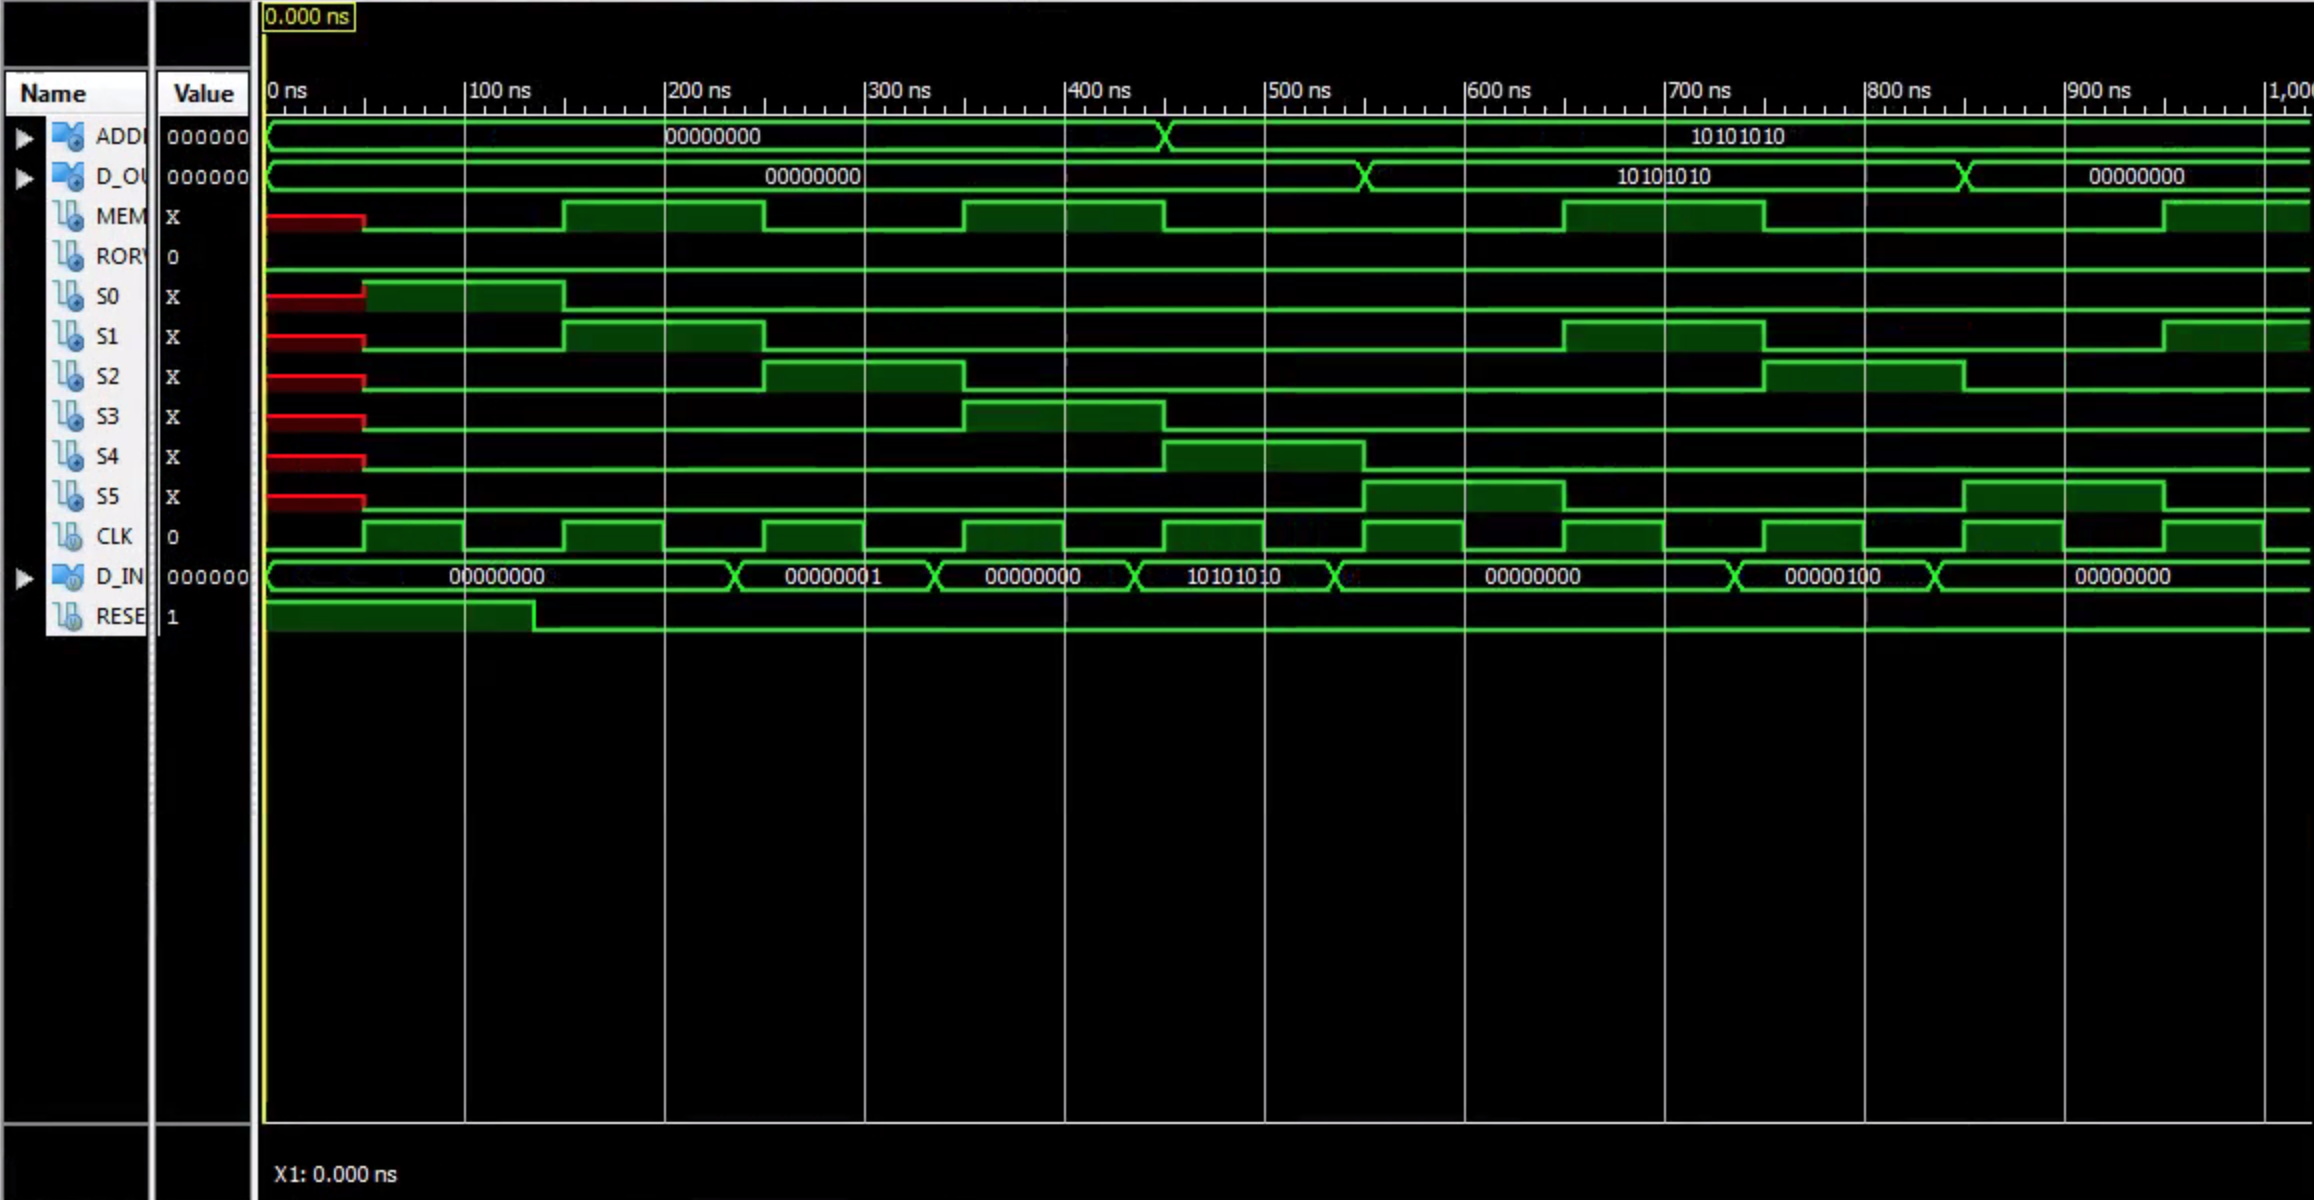
\includegraphics[scale=.35]{c1.png}\\
	This segment shows a reset followed by adding 170 and clearing.
	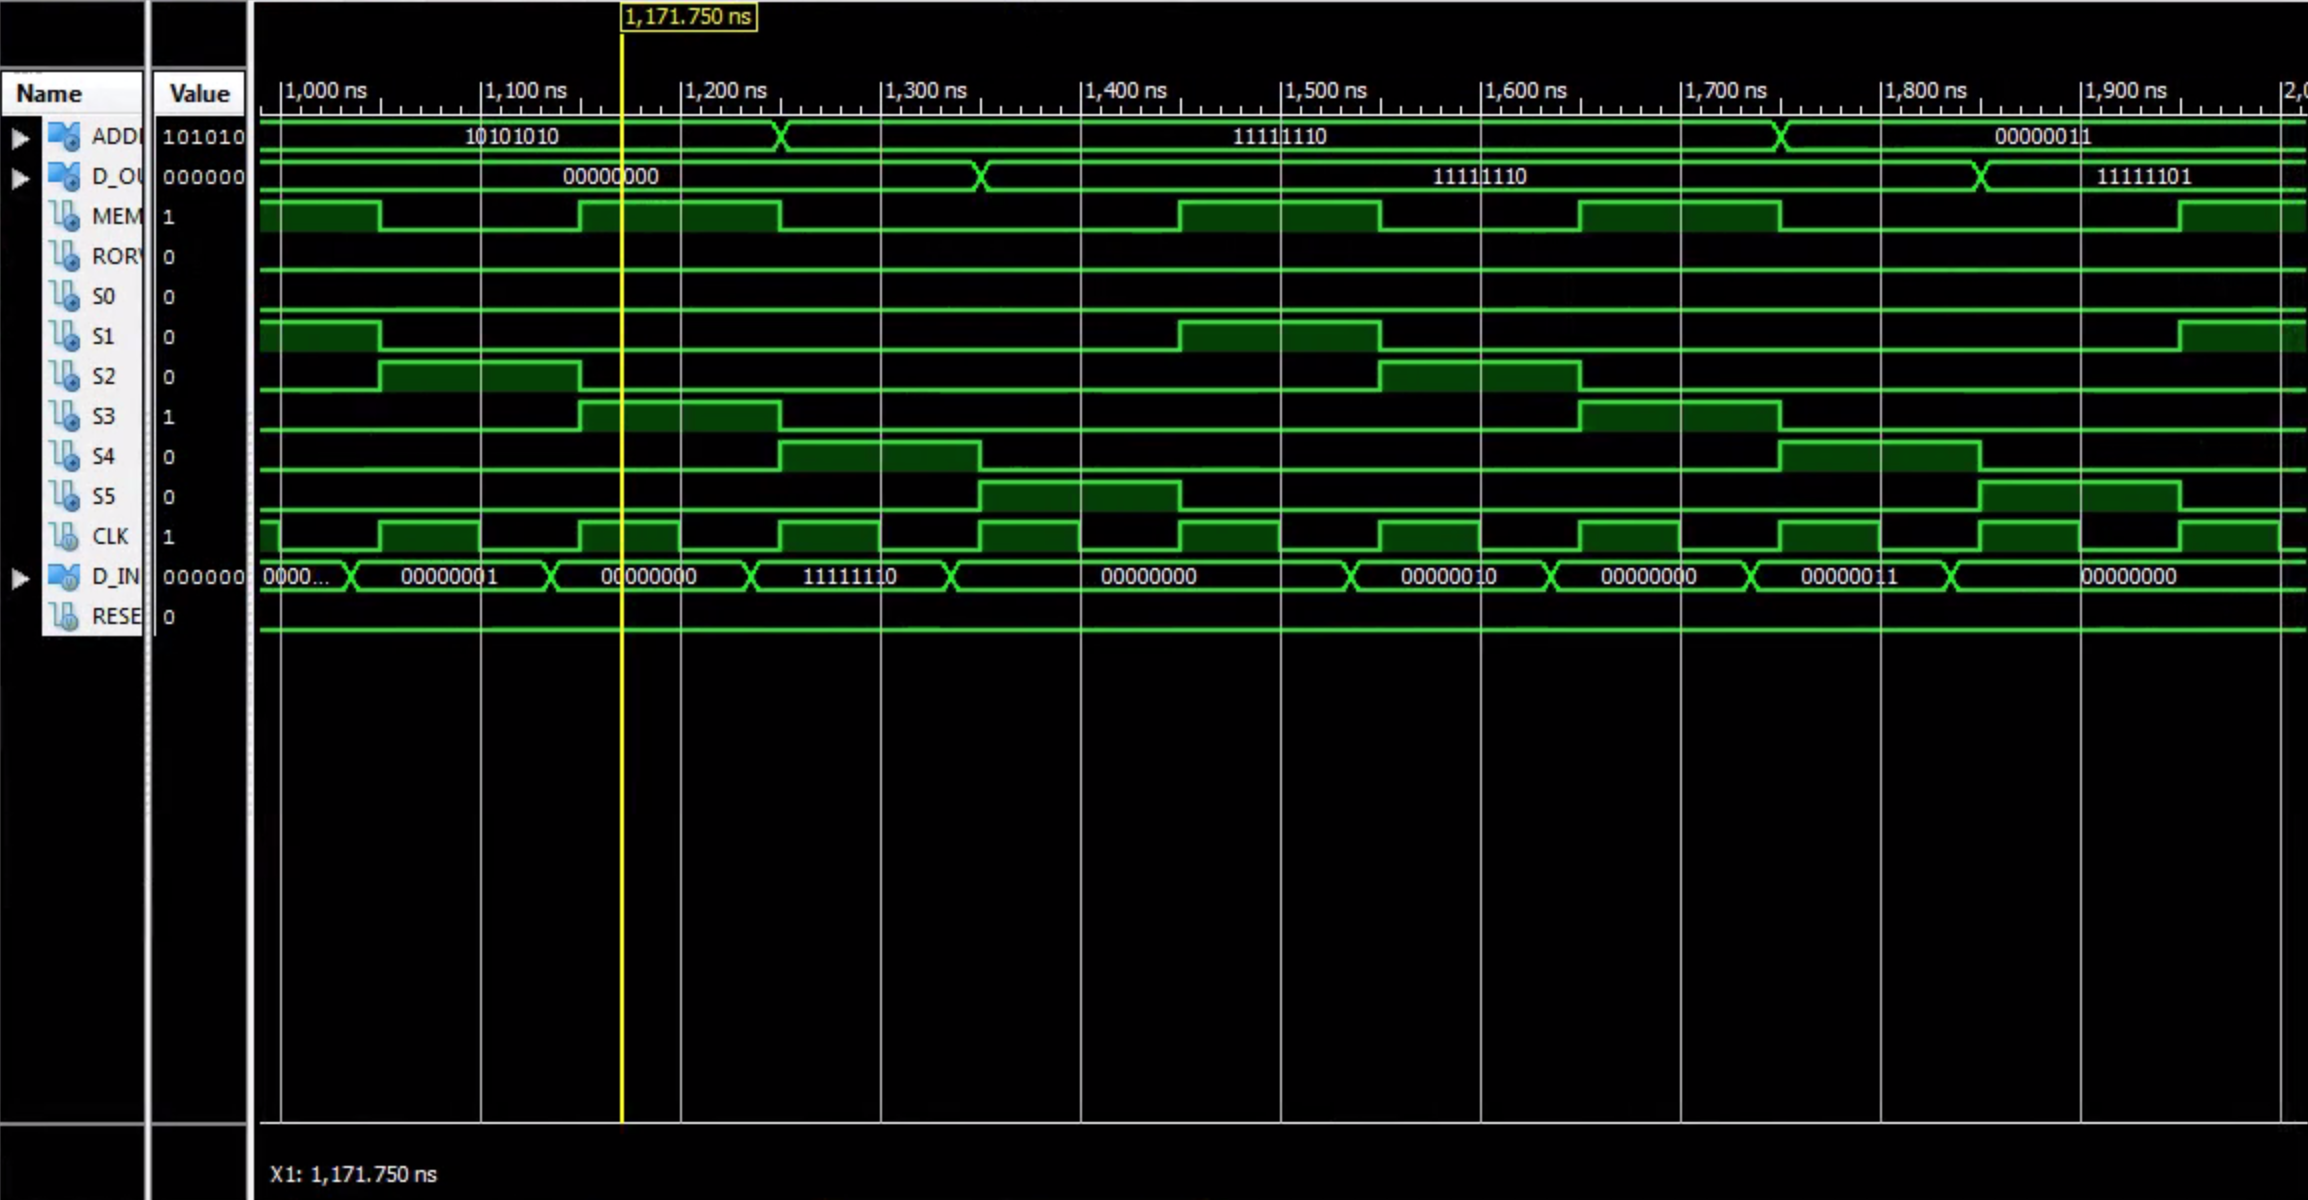
\includegraphics[scale=.35]{c2.png}\\
	This segment shows adding 254 and then subtracting 3 leaving 251 which can be seen at the beginning of the next segment.
	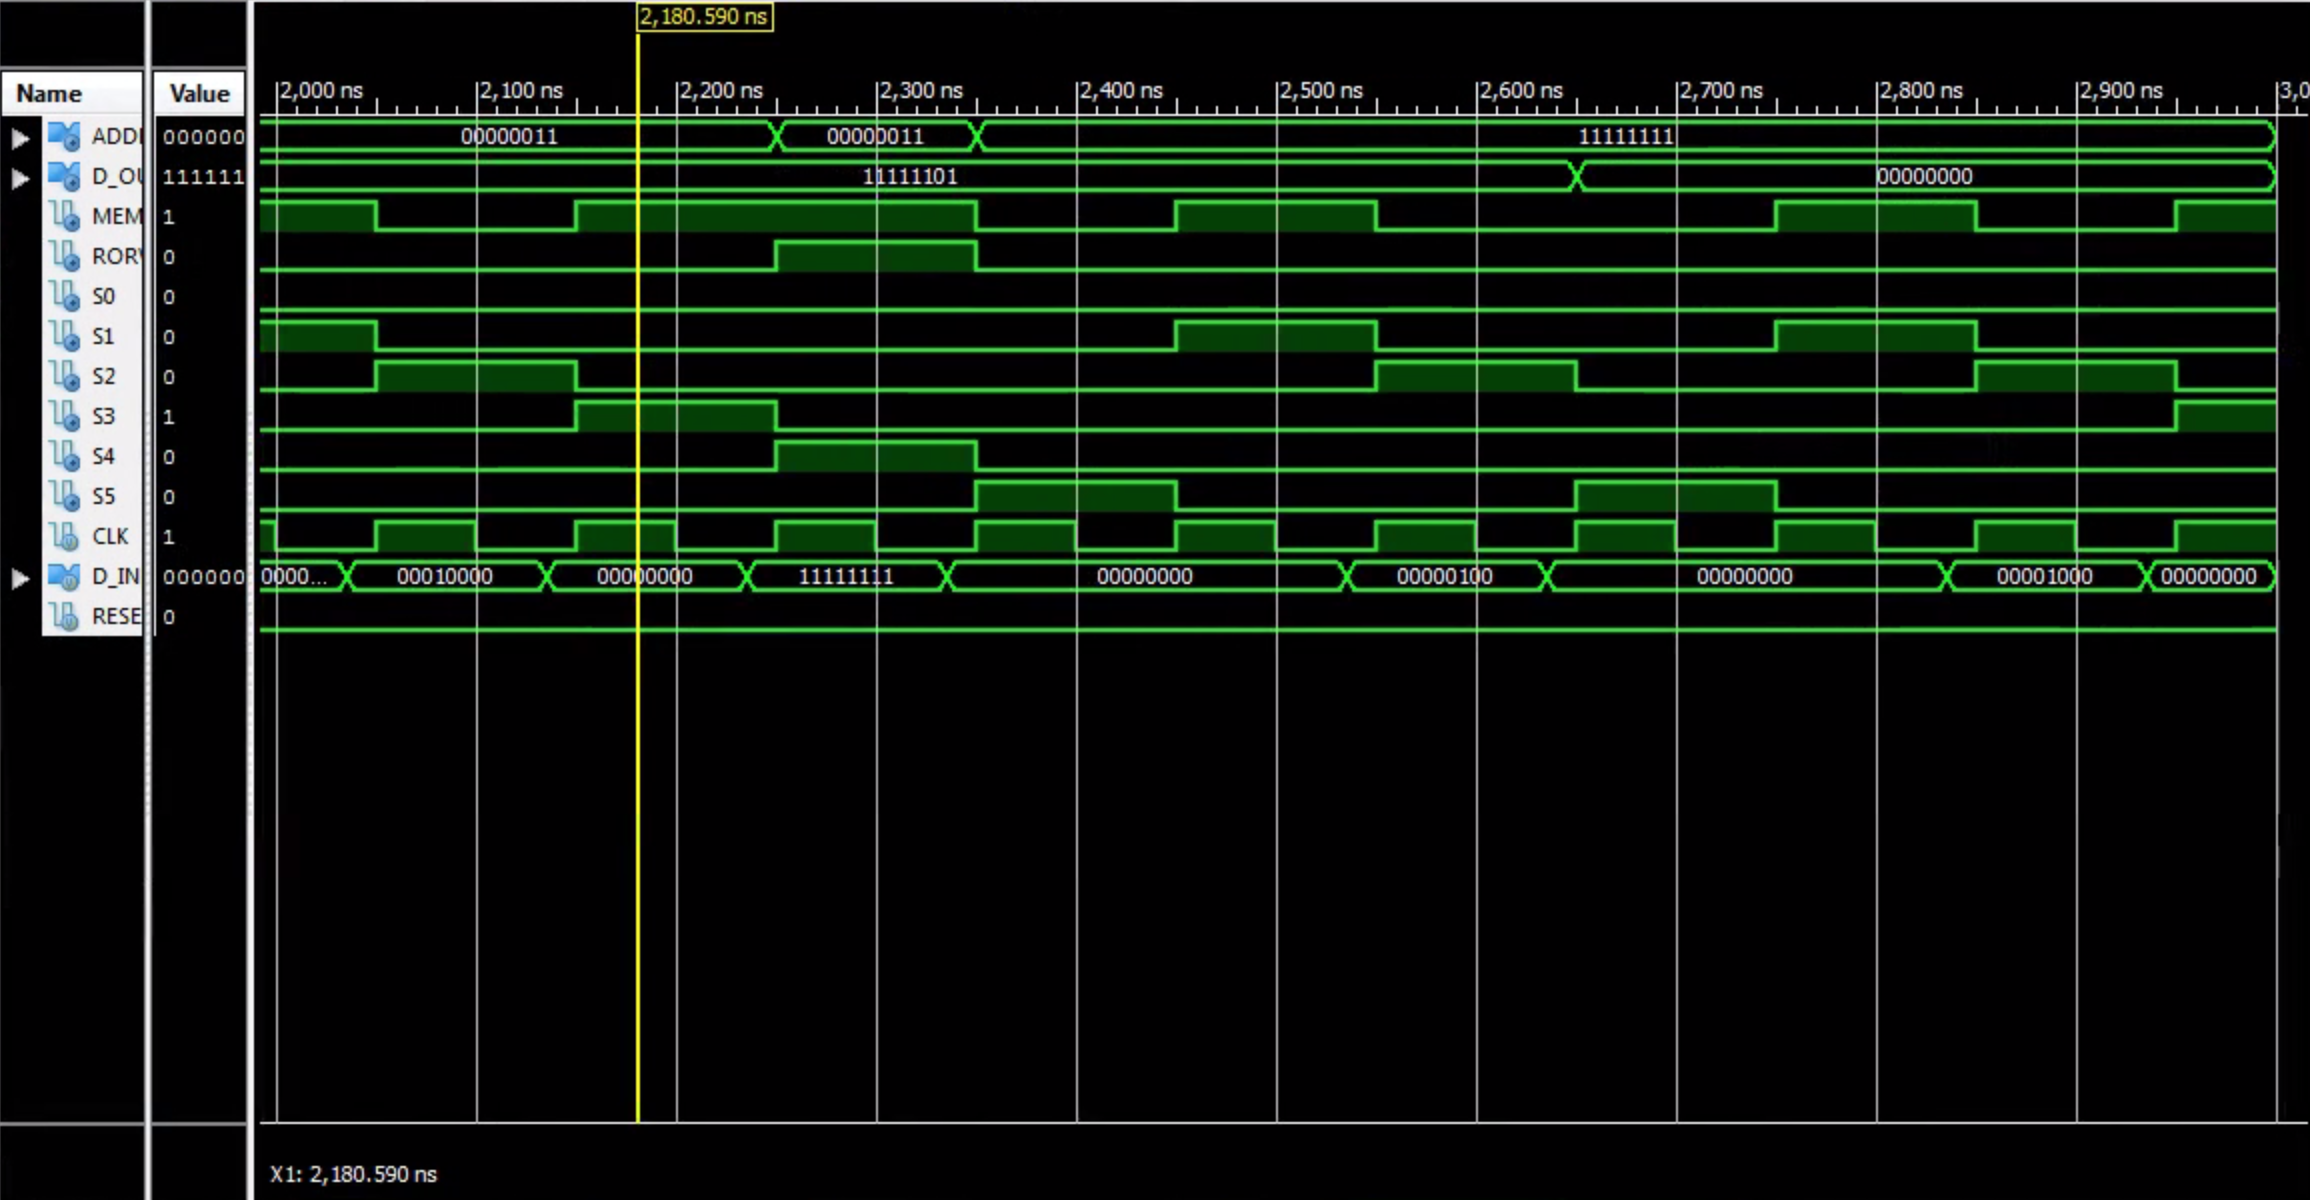
\includegraphics[scale=.35]{c3.png}\\
	This segment begins with a store of the answer previous to the address 255. Then a clear and we branch if not zero to 11001100 which can be seen in the next segment.
	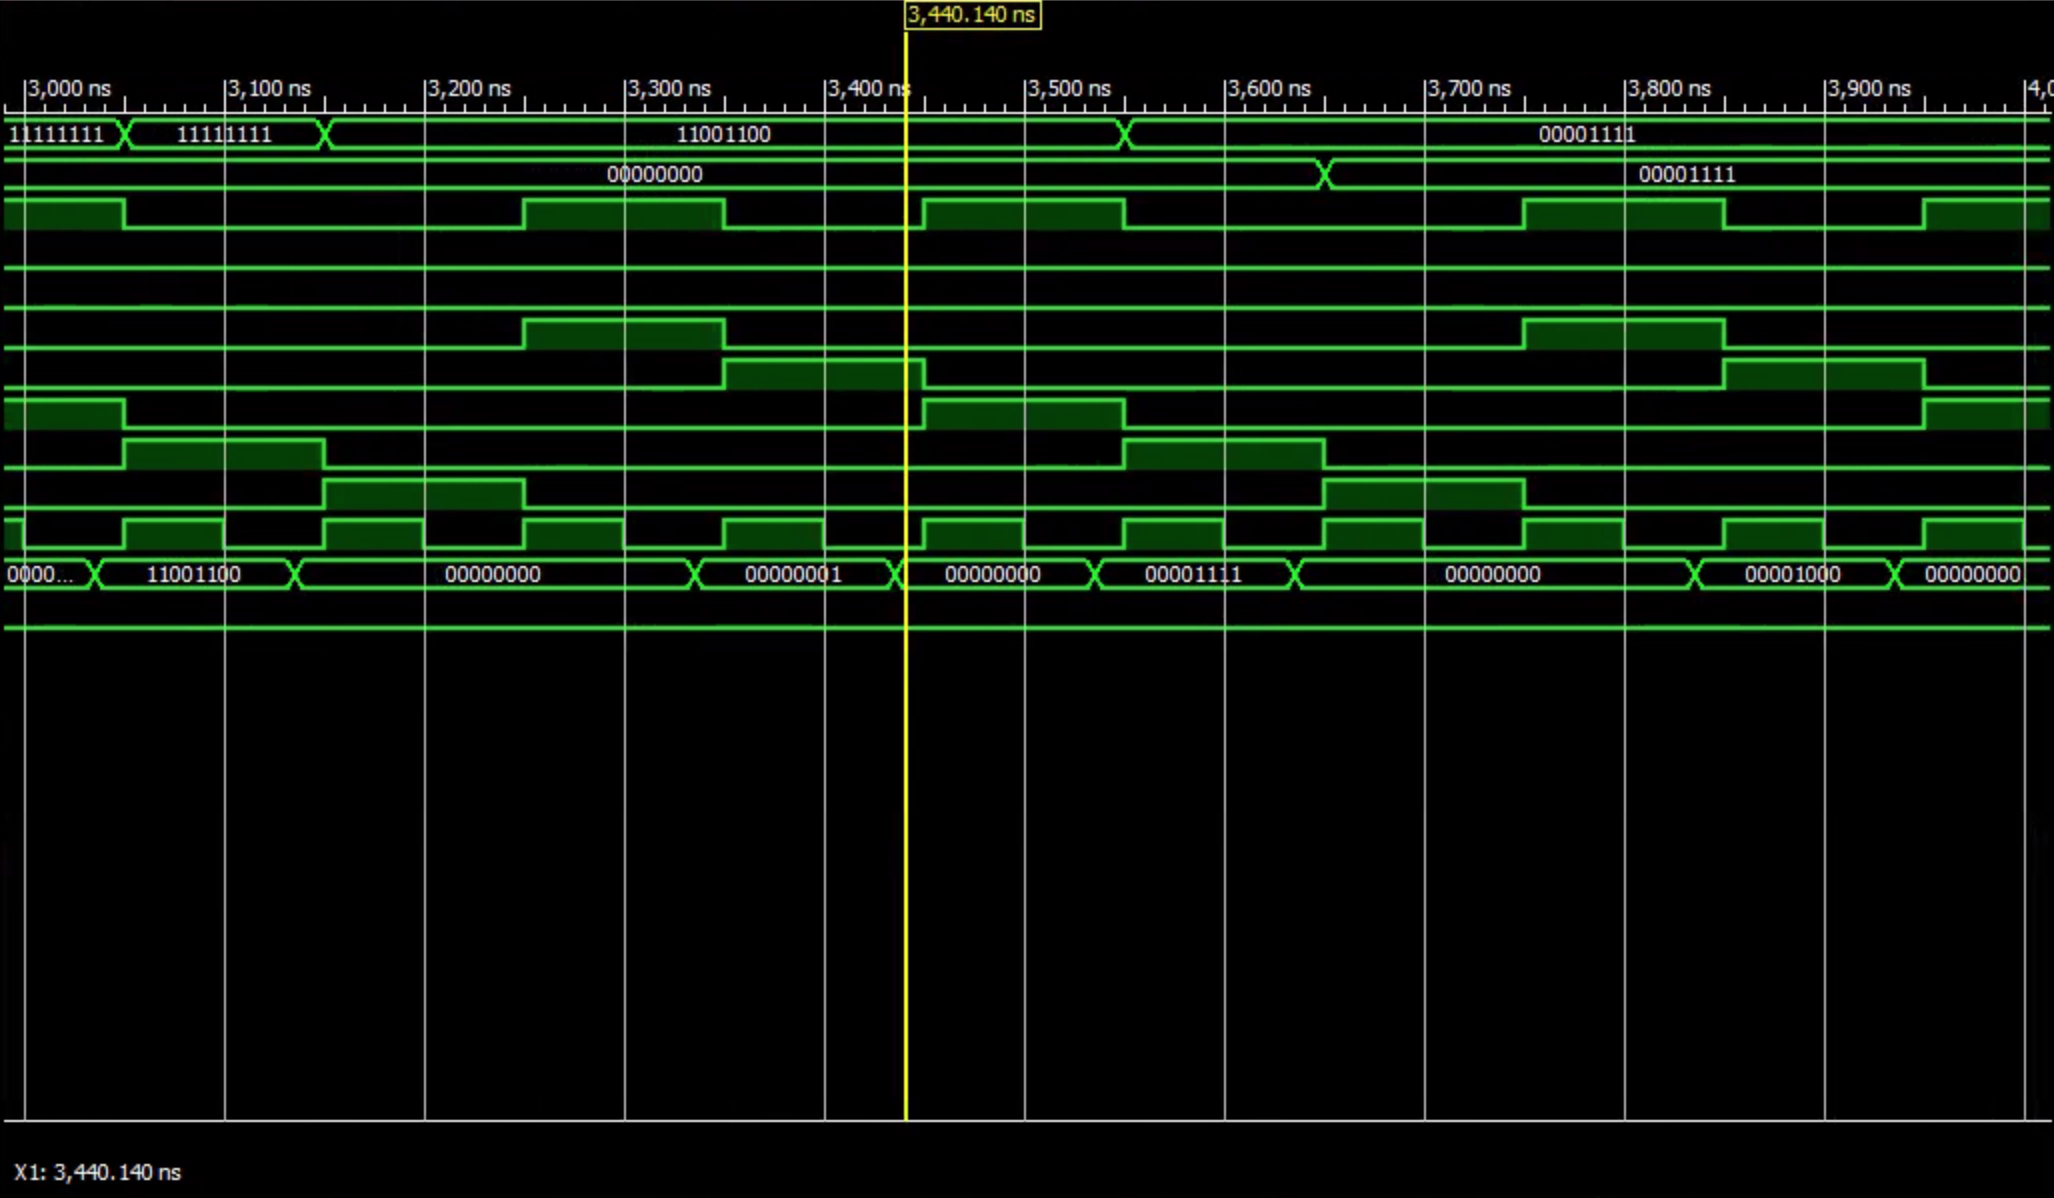
\includegraphics[scale=.35]{c4.png}\\
	Finally we clear add 15 and branch if not zero to 11001100.
\end{center}

	\newpage
\section{Significance} \vspace{-.7cm} \line(1,0){470}
	\paragraph{} 
		With the toy processor now built we can now execute very simple programs including tasks like add, subtract, clear, branch if not zero, and store. To improve its use, we can implement more features like ROM and RAM paths in order to execute more complex programs, and bring the whole implementation to the board. 

 \section{Comments/Suggestions}\vspace{-.7cm} \line(1,0){470}
 	\paragraph{} 
 		N.A.
		
\end{document}


